\begin{figure}[!htbp]
  \centering
  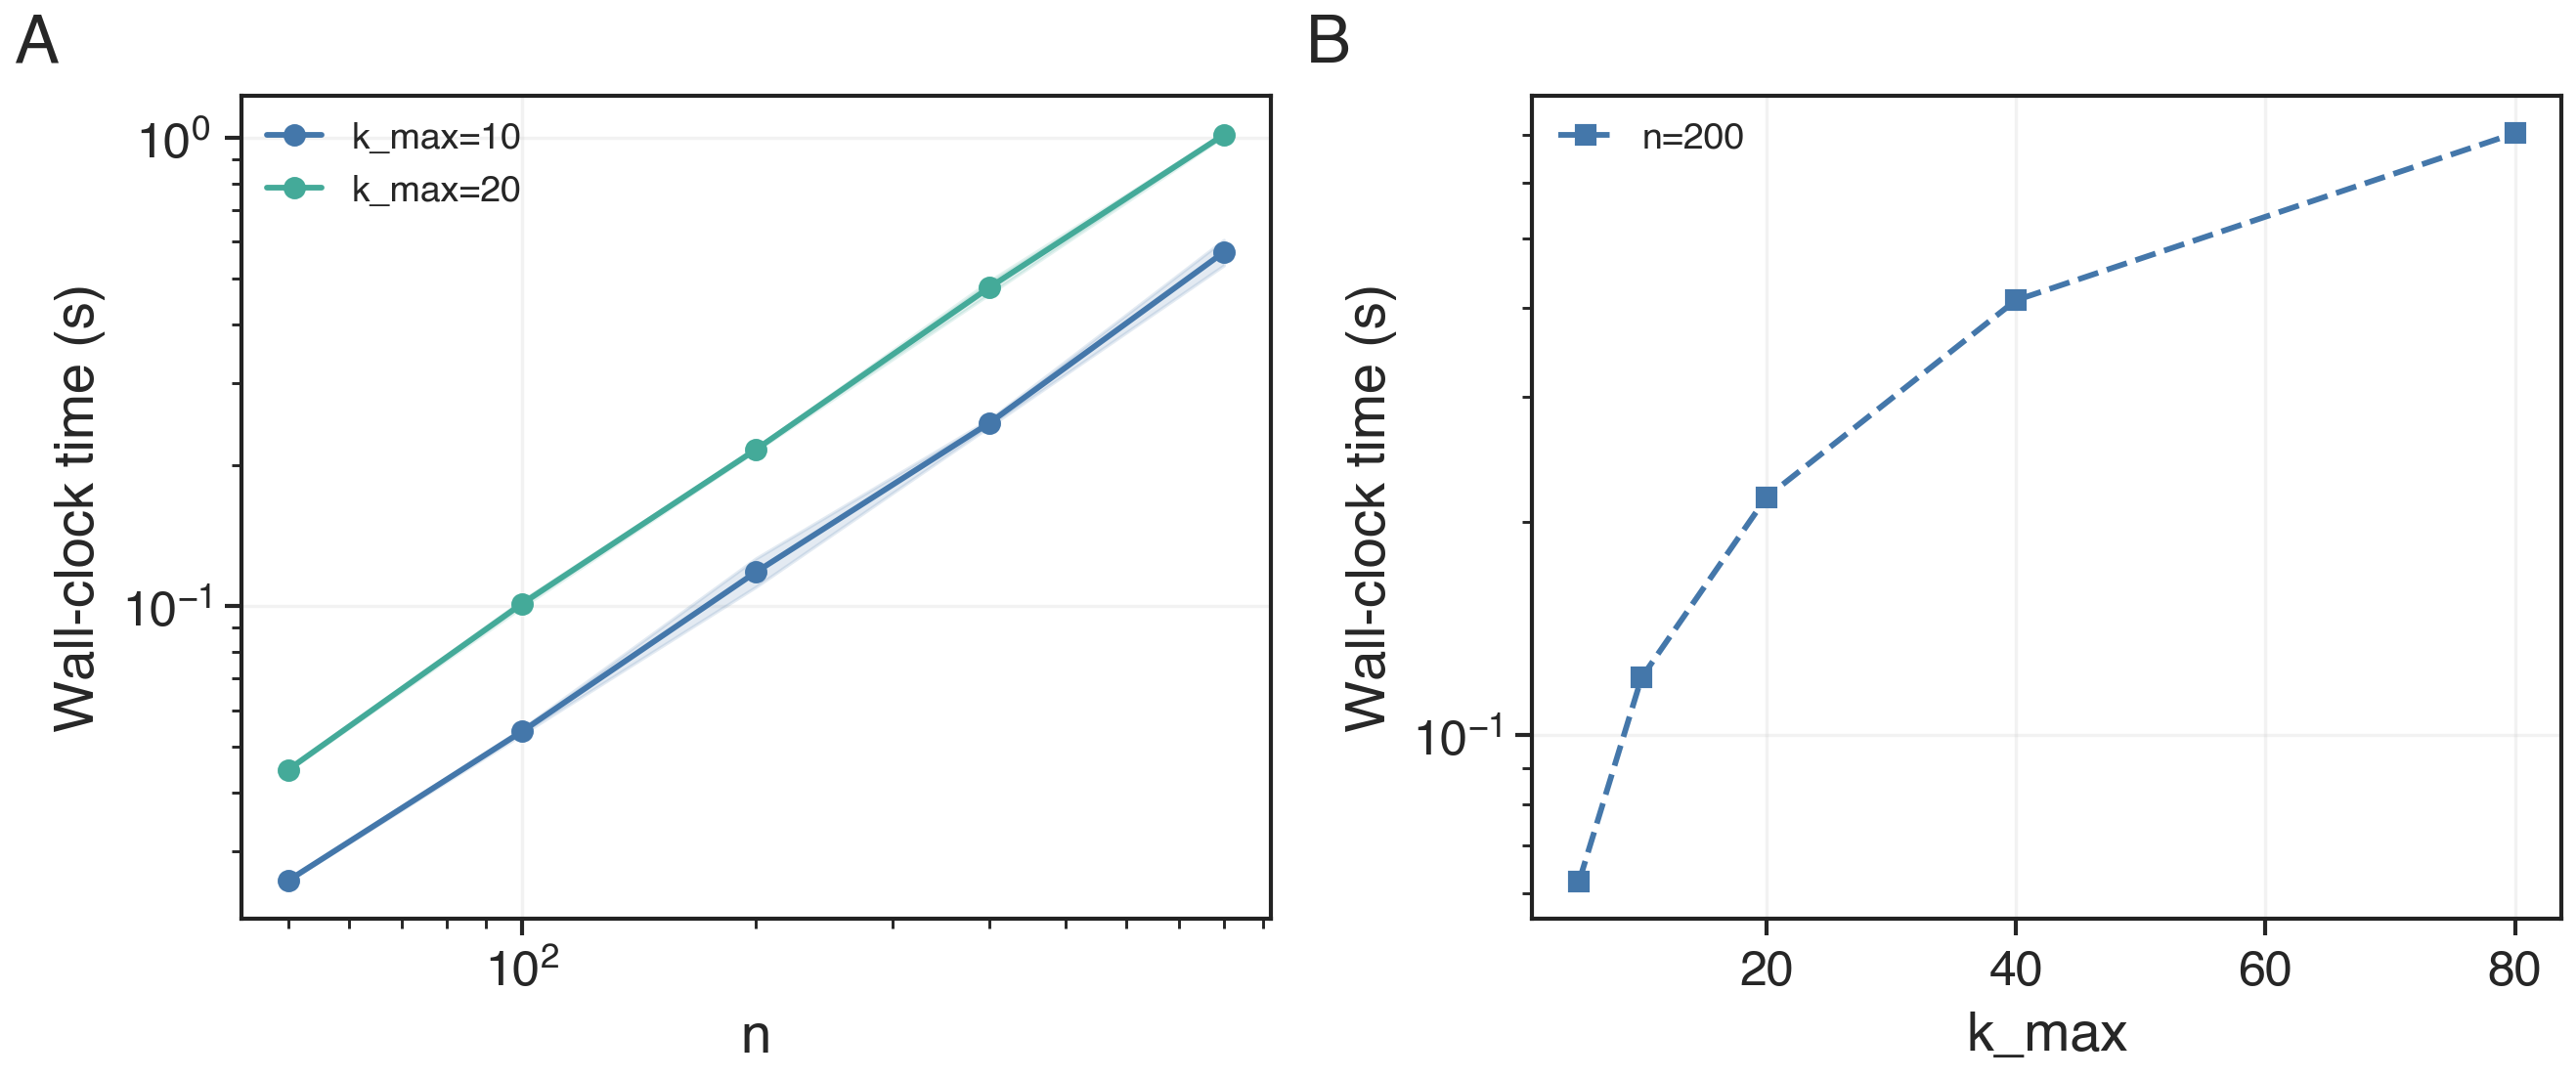
\includegraphics[width=0.92\textwidth,height=0.67\textheight,keepaspectratio]{paper/figures/fig5_runtime_scaling.png}
  \caption{Gaussian runtime measurements. Points are means over five repetitions
    and error bars are one standard deviation. Dashed references show
    quadratic-in-$n$ and linear-in-$k_{\max}$ guides, not fitted complexity claims.}
  \label{fig:runtime-result-paper}
\end{figure}
